\chapter{Implementation}
\label{chap:num_5}

The following chapter is going to cover the implementation of \lpas{} package, the frontend components as well as the ontology. The first part of the chapter dedicated to the implementation of the package will provide a detailed overview of the decisions made on the development stack, the main challenges invoked in refactoring the original \lpa{} codebase, and making the \solid{} related functionality more generic. The frontend components section will dive deeper into the implementation of the mocks provided in \autoref{chap:num_4}, main decisions, and challenges while developing under React. The ontology section will describe how the designed \lpas{} vocabulary was converted into a \texttt{.owl} file, converted into \texttt{.jsonld} Schema and later integrated into the \lpa{} frontend. Lastly, an overview of the implementation results will be presented by reiterating over the defined \lpa{} requirements and how they were satisfied by the implementation.
 
\section{Storage Package}

The initial implementation of \lpa{} frontend was written in \texttt{JavaScript ES6} \footnote{http://es6-features.org} and \texttt{React} framework. The development stack also included tools such as \texttt{Babel} \footnote{https://babeljs.io} compiler and \texttt{Webpack} \footnote{https://webpack.js.org} package bundler. As the amount of features and functionality to cover was increasing, the decision was made to separate the \solid{} storage related functionality into a separate \texttt{npm} package and call it \lpas{}. This section will provide an overview of preliminaries chosen for the implementation of \lpas{} package as well as the specifics of implementations of each abstraction defined in \autoref{ssec:storage}. 

\subsection{Preliminaries}

As briefly mentioned earlier, there several main libraries used inside the \lpas{} package:

\begin{itemize}
    \item \texttt{rdflib} is a low-level RDF library, that mainly provides the functionality to Read and Write RDF in many popular formats, a querying store and an ability to use SPARQL queries.
    \item \texttt{solid-auth-client}, a browser library that implements \solid{} specifications for providing authentication. This is the main library used to enable the authentication into \lpa{} platform.    
%    Todo add ref for testing chapter
    \item \texttt{ava.js}, is a simple JavaScript unit tests runner with TypeScript support. More on testing will be described in a Testing chapter. It is important to note that proper unit testing was one of the other major factors for splitting the \solid{} functionality into a separate package. Easier code maintainability, along with features of TypeScript, significantly improved test-driven development of the package. 
    \item \texttt{istanbul.js}, a test coverage tool used along with \texttt{ava.js}. The library provides a convenient command-line interface that was used for improving Continuous Integration and Delivery jobs. More details on CI and CD are covered in the testing chapter.
\end{itemize}

Due to the complexity of the usage of the stated libraries, specifically \texttt{rdflib}, having an environment and a language that provides a fully-featured object-oriented programming and static type-checking would directly affect the code maintainability and usage. Hence, the codebase of \lpas{} was implemented using \texttt{TypeScript} \footnote{https://www.typescriptlang.org}. TypeScript is a strict syntactical superset of JavaScript that provides optional static typing and better object-oriented programming capabilities.  

\begin{figure}[h]
\centering
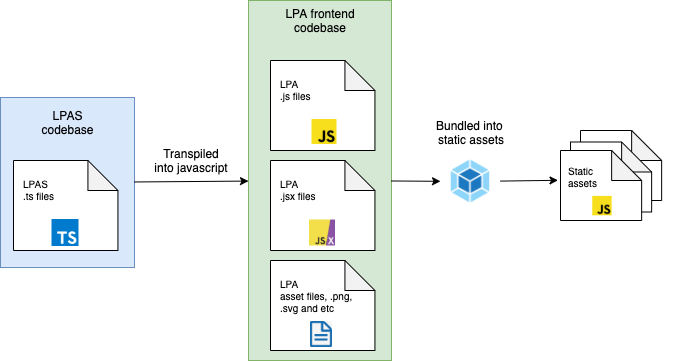
\includegraphics[width=12cm]{lpas_implementation_transpilation_diagram.png}
\caption{A diagram demonstrating the process of transpilation of \lpas{} package and bundling \lpa{} frontend with Webpack}
\label{fig:lpas_implementation_transpilation_diagram}
\end{figure}

As demonstrated on \autoref{fig:lpas_implementation_transpilation_diagram}, integrating the package into the \lpa{} codebase was done using the TypeScript compiler that allows transpilation into ES6 compatible Javascript syntax. The package, as well as the rest of the \lpa{} codebase,  is later bundled into a set of static assets using Webpack. The assets mainly consist of a set of media files such as \texttt{.png} and \texttt{.svg} files and a large \texttt{.js} file that contain the whole \lpa{} frontend. One of a few disadvantages with that approach is that the initial loading of the frontend might take a few seconds to load in the browser. Afterward, the interaction with the platform is seamless and does not involve any additional loading.

\subsubsection{Project structure}

The structure of the \lpas{} package is simple and straightforward and can be demonstrated as follows:

\begin{lstlisting}
- build       # Transpiled JS code    
- markdown    # Markdown assets
- src         # Root project folder
  - lib       # Main library codebase
    - common  # Utilities and helper functions
   	- ...     # TypeScript tests and core abstractions
  - types     # Custom user-defined type definitions
- docs        # Static html with library documentation
_ ...         # Readme and various configuration files
\end{lstlisting}

The proceeding sections will describe the individual abstractions mentioned in \autoref{ssec:storage} section.

\subsection{Authentication Manager}

This section will continue the architectural description of the Authentication manager described in \autoref{sssec:authentication_manager}, describe the implementation, and provide examples of how the abstraction is used inside \lpa{}.

The \textit{AuthenticationManager} is a Singleton class, instantiated only once and utilised both in the package itself as well as being invoked from \lpa{} frontend codebase. The reason for the class being implemented as a singleton is due to the fact that it wraps the functionality of \texttt{solid-auth-client} library. Aside from providing the WebID authentication,  \texttt{solid-auth-client} implements a WebID OIDC specific \textit{fetch} functionality. The \textit{FETCH API} is originally a JavaScript API that provides an ability to send asynchronous HTTP calls. The implementation in \texttt{solid-auth-client}, is based on \texttt{isomorpic-fetch}, which is a third party framework that implements the \textit{Fetch API} both for browsers and node.js. Hence, the abstraction is used for:
\begin{itemize}
    \item Authentication, and ability to track the user session with callbacks. 
    \item Sending HTTP calls to \solid{} server.
\end{itemize}


\begin{figure}[h]
\centering
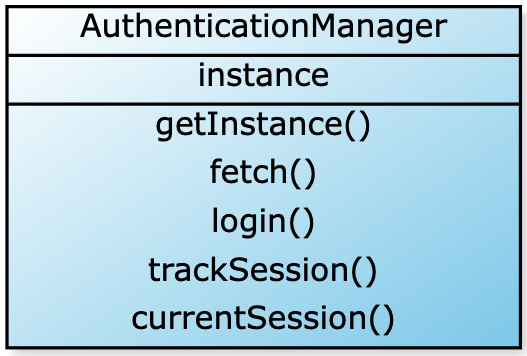
\includegraphics[width=6cm]{lpas_authentication_class.png}
\caption{A class diagram of an implemented AuthenticationManager abstraction}
\label{fig:lpas_authentication_class}
\end{figure}


In other words, once the client is logged in the \solid{} app, consequtive interactions are performed via \textit{fetch} function that is conveniently wrapped in the \textit{AuthenticationManager} abstraction.

As demonstrated on \autoref{fig:lpas_authentication_class}, the class consist of a set of public methods described as follows:
\begin{itemize}
    \item \textit{getInstance()}, this public method returns a singleton instance to an AuthenticationManager.
    \item \textit{fetch()}, a wrapper redirecting the call to \texttt{solid-auth-client} fetch method.
    \item \textit{login()}, a wrapper redirecting the call to \texttt{solid-auth-client} login method.
    \item \textit{trackSession()}, a method with asynchronous callback notifying the listener when a logout or login operation is performed.
    \item \textit{currentSession()}, a method returning the instance of a \texttt{solid-auth-client} Session object that contains relevant information about the authenticated user and his WebID. 
\end{itemize}

Referring back to \autoref{fig:lps_authentication_sequence_diagram}, there are several places in \lpa{} codebase where the \textit{AuthenticationManager} is invoked directly. The implementation of React components will be covered in the proceeding section, but the invocation of the abstraction itself can be described as follows:
\begin{itemize}
    \item \textit{Component layouts} are special high-level react containers that wrap every other container inside \lpa{} frontend. They are differentiated by \textit{public} and \textit{private}. The \textit{private} components reactively monitor the authenticated session of a user and redirect them back to the authentication screen whenever the value of the session becomes \texttt{undefined}. It is important to note that the session object from \textit{AuthenticationManger} is duplicated in \lpa{} frontend as a Redux state. Therefore, any changes in the original session object are reflected on that state and triggers re-rendering of layout components. 
    \item \textit{Authentication component functions}, are the functions being invoked when user attempts to perform the authentication. In other words, this is the input that triggers the flow demonstrated earlier on \autoref{fig:lps_authentication_sequence_diagram}.
    \item \textit{The App router}, the main class in \lpa{} that serves as an entry point and utilizing the \texttt{react-router} \footnote{https://www.npmjs.com/package/react-router} package, contains a function that invokes the \textit{trackSession()} method in \textit{AuthenticationManager}. This directly links to the session object and updates the changes from original session to internal Redux state.
\end{itemize}

The usage of both \textit{currentSession()} and \textit{login()} methods from \textit{AuthenticationManager} can be observed below:
\begin{lstlisting}[language=JavaScript]
login = async (idp, callbackUri) => {
    const session = await AuthenticationManager.currentSession();
    if (!session)
      await AuthenticationManager.login(idp, {
        storage: localStorage
      });
    else {
      Log.info(`Logged in as ${session.webId}`);
      return session;
    }
};
\end{lstlisting}

To sum up, the \textit{AuthenticationManager} is a simple and straightforward singleton abstraction that wraps the \texttt{solid-auth-client} library and only necessary functions from the wrapped library to be used inside \lpas{} frontend. The examples of invocation from within the \lpas{} package are limited to directly calling the \textit{fetch()} method whenever an HTTP request is assembled and needs to be executed, more details on that will be described in a section dedicated to \textit{FileManager} abstraction.  

\section{File Manager}

\section{Access Control Manager}


%TODO: Sections belows are WIP

\section{Hosting Storage Ontology}


\section{Storage Frontend}

\begin{lstlisting}[language=json]
{
  "@graph": [
    {
      "@id": "https://w3id.org/def/lpapps",
      "@type": "https://w3id.org/def/lpapps#VisualizerConfiguration",
      "https://w3id.org/def/lpapps#applicationData": "undefined",
      "https://w3id.org/def/lpapps#author": {
        "@id": "https://w3id.org/profile/card#me"
      },
      "https://w3id.org/def/lpapps#backgroundColor": "#671570",
      "https://w3id.org/def/lpapps#configurationId": "1afbe0f2-3a58-424e-91ec-6a41ae8717b3",
      "https://w3id.org/def/lpapps#endpoint": "chord",
      "https://w3id.org/def/lpapps#etlExecutionIri": "http://localhost:8080/resources/executions/1574612566772-0-2f47c643-55c0-419d-9313-1381cec14b1d",
      "https://w3id.org/def/lpapps#filteredBy": {
        "@id": "_:b0"
      },
      "https://w3id.org/def/lpapps#graphIri": "https://applications.linkedpipes.com/graph/84b34afd-6990-411a-920e-cb402b29797f-16dd6a86-2743-42cb-aea7-368b14aa0eff",
      "https://w3id.org/def/lpapps#published": "2019-11-24T16:27:51.043Z",
      "https://w3id.org/def/lpapps#title": "Chord application",
      "https://w3id.org/def/lpapps#visualizerType": "CHORD"
    }
  ]
}
\end{lstlisting}

\section{Implementing requirements}